\documentclass[a4paper,12pt,oneside]{book}

%-------------------------------Start of the Preable------------------------------------------------
\usepackage[english]{babel}
\usepackage{blindtext}
%packagr for hyperlinks
\usepackage{hyperref}
\hypersetup{
    colorlinks=true,
    linkcolor=blue,
    filecolor=magenta,      
    urlcolor=cyan,
}

\urlstyle{same}
%use of package fancy header
\usepackage{fancyhdr}
\setlength\headheight{26pt}
\fancyhf{}
%\rhead{
\includegraphics[width=1cm]{logo}}
\lhead{\rightmark}
\rhead{
\includegraphics[width=1cm]{logo}}
\fancyfoot[RE, RO]{\thepage}
\fancyfoot[CE, CO]{\href{http://www.e-yantra.org}{www.e-yantra.org}}

\pagestyle{fancy}

%use of package for section title formatting
\usepackage{titlesec}
\titleformat{\chapter}
  {\Large\bfseries} % format
  {}                % label
  {0pt}             % sep
  {\huge}           % before-code
 
%use of package tcolorbox for colorful textbox
\usepackage[most]{tcolorbox}
\tcbset{colback=cyan!5!white,colframe=cyan!75!black,halign title = flush center}

\newtcolorbox{mybox}[1]{colback=cyan!5!white,
colframe=cyan!75!black,fonttitle=\bfseries,
title=\textbf{\Large{#1}}}

%use of package marginnote for notes in margin
\usepackage{marginnote}

%use of packgage watermark for pages
%\usepackage{draftwatermark}
%\SetWatermarkText{
\includegraphics{logo}}
\usepackage[scale=2,opacity=0.1,angle=0]{background}
\backgroundsetup{
contents={
\includegraphics{logo}}
}

%use of newcommand for keywords color
\usepackage{xcolor}
\newcommand{\keyword}[1]{\textcolor{red}{\textbf{#1}}}

%package for inserting pictures
\usepackage{graphicx}

%package for highlighting
\usepackage{color,soul}

%new command for table
\newcommand{\head}[1]{\textnormal{\textbf{#1}}}


%----------------------End of the Preamble---------------------------------------


\begin{document}

%---------------------Title Page------------------------------------------------
\begin{titlepage}
\raggedright
{\Large eYSIP2017\\[1cm]}
{\Huge\scshape MiniBOT Blockly \\[.1in]}
\vfill
\begin{flushright}
\textbf{\large Intern 1 \\}
{\large Hitesh Tewani \\}
\textbf{\large  Mentors  \\}
{\large 1.Deepa Avadiappan\\}
{\large 2.Rutuja Ekatpure \\}

{\large Duration of Internship: $ 22/05/2017-07/07/2017 $ \\}
\end{flushright}

{\itshape 2017, e-Yantra Publication}
\end{titlepage}
%-------------------------------------------------------------------------------

\chapter[Project Tag]{Firebird 5 Blockly- New Blocks}
\section*{Abstract}
Three New blocks have been added to firebird 5 Blockly which include Xbee (TX and RX), Bluetooth( TX and RX) and Servo Motor blocks.


\section{Block Description}
\subsection{Bluetooth and Xbee Transmit}
    \begin{center}
    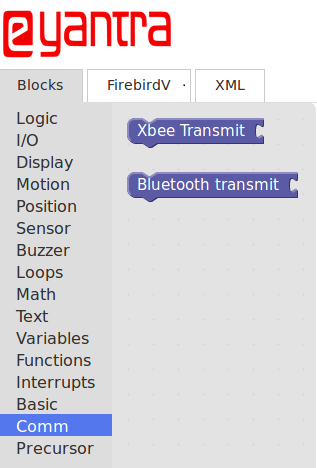
\includegraphics[scale =0.6]{xbtransm}\\[.3in]
    \textbf{Bluetooth and Xbee transmit}\\[1.3in]
    \end{center}
    New Block named Comm (Communication) was introduced in Blocks section of Firebird 5 Blockly. This block contains two sub blocks named Xbee Transmit and Bluetooth transmit to which a math block or string block can be attached in order to transmit data from firebird 5 to other xbee or bluetooth receiving device configured with the transmitting device on firebird 5. 
\subsection{Bluetooth and Xbee Receive}
    \begin{center}
    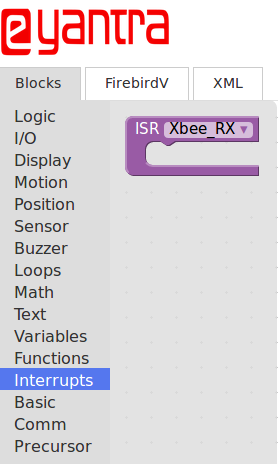
\includegraphics[scale =0.6]{xbrec}\\[.3in]
    \textbf{Bluetooth and Xbee receive}\\[1.3in]
    \end{center}
    ISR Block was modified. Earlier it had subsection where vector and attribute could be entered but now it has been provided with a drop down menu which consist of Xbee Receive, Bluetooth Receive and Interrupt Switch. Xbee Receive and Bluetooth Receive are functional blocks which are able to receive string data from other transmitting devices with which they are configured.   
\subsection{Servo and servo free}    
    \begin{center}
    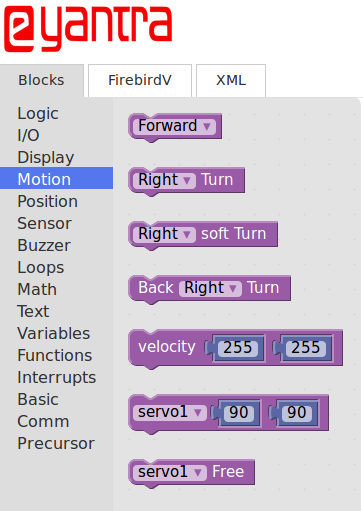
\includegraphics[scale =0.6]{servob}\\[.3in]
    \textbf{Servo and Servo free}\\[1.3in]
    \end{center}
    Motion block has been updated with two sub blocks named Servo Motor and Servo Free. Servo Motor Block has a drop-down where user can select servo motor of his choice i.e servo1, servo2 or servo3. Similarly he can choose servo free block for servo(1,2 or 3) to reduce power consumption by servo motor when work is done.
\subsection{Initialization Block}    
    \begin{center}
    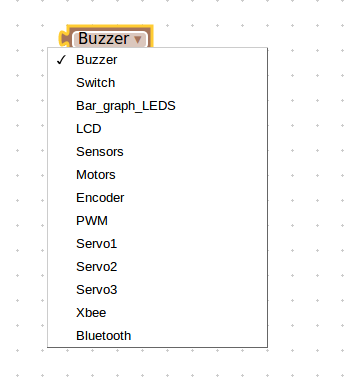
\includegraphics[scale =0.6]{initb}\\[.3in]
    \textbf{Initialization Block Updated}\\[1.3in]
    \end{center}
    New blocks introduced in Firebird 5 Blockly can be initialized by selecting them from drop down of initialize which is a subsection present in Basic block section of Firebird 5 Blockly. The updated drop-down includes Xbee, Bluetooth and servo(1,2 and 3) sections.
\newpage\subsection{Do Nothing}    
    \begin{center}
    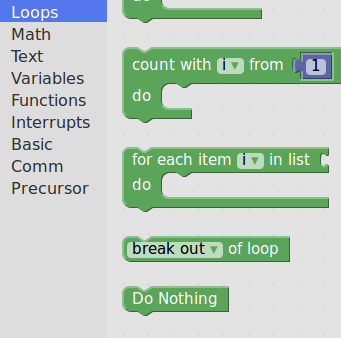
\includegraphics[scale =0.6]{Dono}\\[.3in]
    \textbf{Do Nothing}\\[1.3in]
    \end{center}
    This block is used to keep the microcontroller busy in order to receive interrupts.

\newpage\section{Examples of new blocks}    
    
\begin{center}
    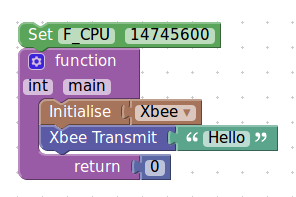
\includegraphics[scale =0.6]{xbeetxsam}\\[.3in]
    \textbf{Xbee Transmit}\\[1.3in]
    \end{center}
    \vspace{-2cm}
    Above is a algorithm to set up blocks in blockly for Xbee to transmit a string
    data as in here it transmits string "hello".    
\begin{center}
    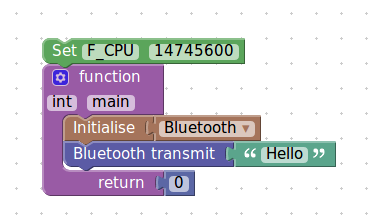
\includegraphics[scale =0.6]{blutxsam1}\\[.3in]
    \textbf{Bluetooth Transmit}\\[1.3in]
    \end{center}
    \vspace{-2cm}
    Above is a algorithm to set up blocks in blockly for Bluetooth to transmit a string data as in here it transmits string "hello".
    
\begin{center}
    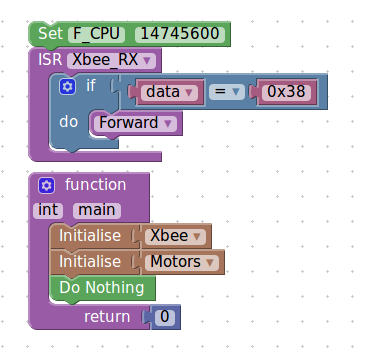
\includegraphics[scale =0.6]{xbeerecimp}\\[.3in]
    \textbf{Xbee Receive}\\[1.3in]
    \end{center}
    \vspace{-2cm}
    Above is the example of how xbee can be set up to receive data from other configured device and then accordingly be used to perform certain task based upon the data received. 
    
\begin{center}
    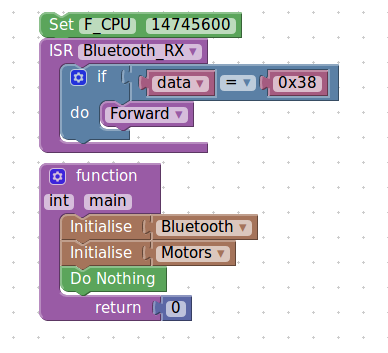
\includegraphics[scale =0.6]{blerecimp}\\[.3in]
    \textbf{Bluetooth Receive}\\[1.3in]
    \end{center}
    \vspace{-2cm}
    Above is the example of how Bluetooth can be set up to receive data from other configured device and then accordingly be used to perform certain task based upon the data received.
    
\begin{center}
    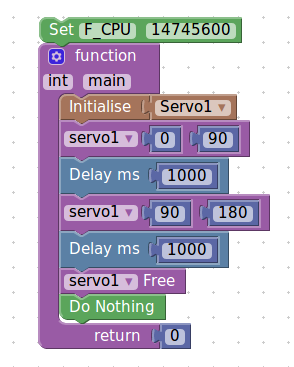
\includegraphics[scale =0.6]{servosam}\\[.3in]
    \textbf{Servo Motor}\\[1.3in]
    \end{center}
    \vspace{-2cm}
    Now above blocks represent a algorithm in which servo motor is first initialized to rotate from 0 to 90 deg and then wait for a sec and then again rotate from 90 to 180 deg. After rotation servo motor is left free so that it does not consume power unnecessarily 

\end{document}

